%
% $RCSfile: logic_manipulates_state.tex,v $
%
% Copyright (C) 2002-2008. Christian Heller.
%
% Permission is granted to copy, distribute and/or modify this document
% under the terms of the GNU Free Documentation License, Version 1.1 or
% any later version published by the Free Software Foundation; with no
% Invariant Sections, with no Front-Cover Texts and with no Back-Cover
% Texts. A copy of the license is included in the section entitled
% "GNU Free Documentation License".
%
% http://www.cybop.net
% - Cybernetics Oriented Programming -
%
% http://www.resmedicinae.org
% - Information in Medicine -
%
% Version: $Revision: 1.1 $ $Date: 2008-08-19 20:41:07 $ $Author: christian $
% Authors: Christian Heller <christian.heller@tuxtax.de>
%

\subsection{Logic Manipulates State}
\label{logic_manipulates_state_heading}
\index{Logic Manipulating State}
\index{Random Access Memory}
\index{RAM}
\index{Knowledge Model}
\index{Knowledge Template}
\index{State Knowledge}
\index{Logic Knowledge}
\index{Static Rule}
\index{Dynamic Behaviour}
\index{Model View Controller}
\index{MVC}
\index{Hierarchical Model View Controller}
\index{HMVC}
\index{MVC Triad}
\index{Knowledge Tree}
\index{Concept}
\index{Unidirectional Dependency}
\index{Data Mapper Pattern}
\index{Data Transfer Object Pattern}
\index{DTO}
\index{Workflow}
\index{Meta Programming}

Knowledge models of the form introduced in chapter \ref{knowledge_schema_heading}
are stored as tree structure in \emph{Random Access Memory} (RAM). They are the
dynamic result of instantiating static knowledge templates (concepts), and hence
changeable. Because knowledge models are passive, they need to be managed by an
active system, responsible for their creation and destruction, as described in
chapter \ref{statics_and_dynamics_heading}.

As the previous sections of this chapter have shown, there are two kinds of
knowledge: \emph{States} and \emph{Logic}. While the former may be placed in a
spatial dimension, the latter are processed as sequence over time. Often, logic
is labelled \emph{dynamic} behaviour -- but only the \emph{execution} of a rule
of logic is dynamic, \emph{not} the rule itself. The rule is \emph{static}.

Rules of logic manipulate input/ output (i/o) states, or more concrete: they
translate input- into output states (section \ref{system_heading}). What
characterises a system is how it applies logic knowledge in order to translate
state knowledge. Yet how to imagine a knowledge model consisting of state- as
well as logic parts? The famous \emph{Model View Controller} (MVC) pattern was
introduced in section \ref{model_view_controller_heading} and reviewed once
more in section \ref{model_view_controller_reflection_heading}. The
\emph{Hierarchical MVC} (HMVC) of section
\ref{hierarchical_model_view_controller_heading} extended the MVC pattern
towards a hierarchy of \emph{MVC Triads}. On that basis, section
\ref{structure_by_hierarchy_heading} demonstrated the omnipresence of
hierarchies in a system.

\begin{figure}[ht]
    \begin{center}
        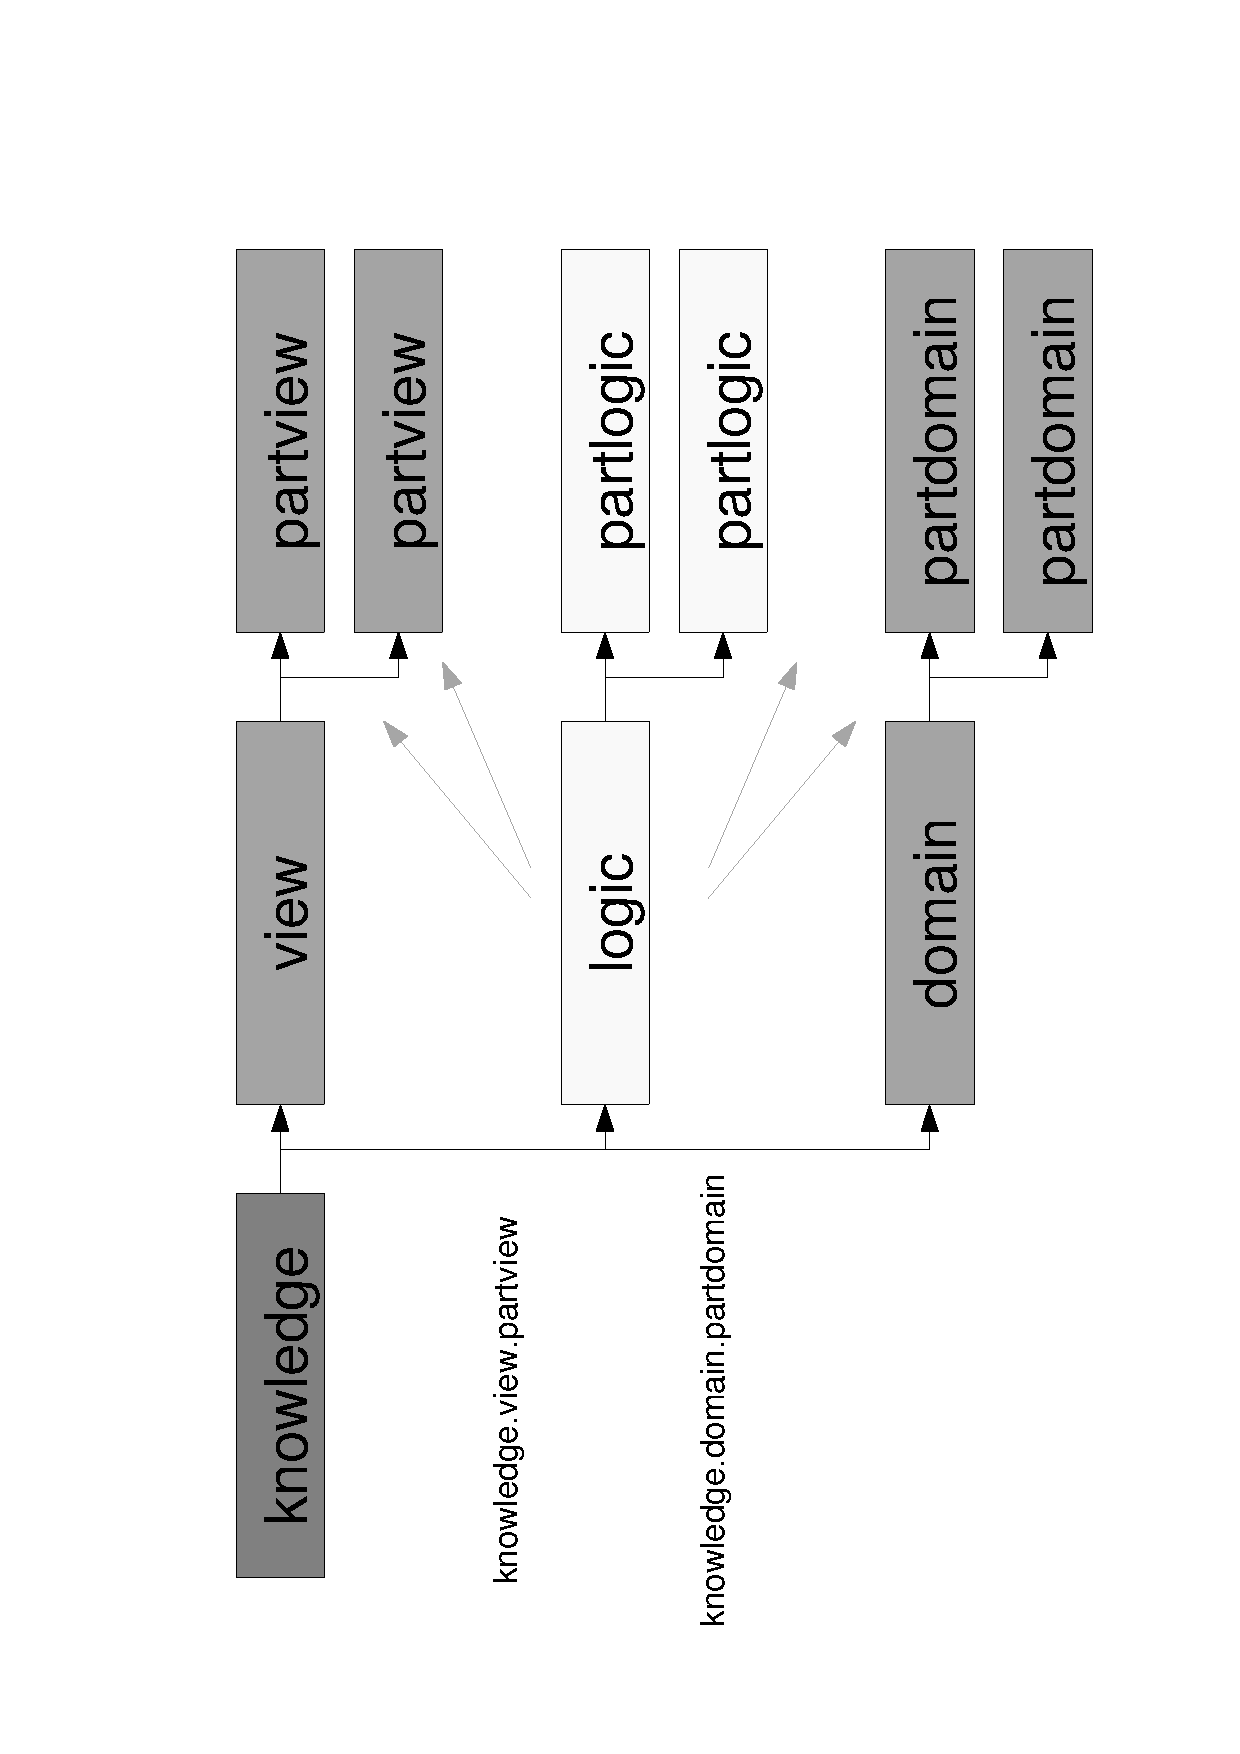
\includegraphics[scale=0.3,angle=-90]{graphic/mvctree.pdf}
        \caption{Runtime Model Hierarchy with Logic manipulating States}
        \label{mvctree_figure}
    \end{center}
\end{figure}

Figure \ref{mvctree_figure} shows the three parts: \emph{Domain} (Model),
\emph{View} and \emph{Logic} (Controller) of the MVC pattern as independent
branches of one common knowledge tree. Each of them represents a concept on its
own. The logic model, however, is allowed to access and change the view- and
domain model; it is able to link different knowledge models, to connect
discrete concepts. But view- and domain model, representing states, are not
allowed to access the logic model. In other words: The dependencies between
logic- and state models are \emph{unidirectional}. New state models such as
textual- or graphical views could be added anytime. All that would be needed to
make a system work with new state models, is the corresponding translation
logic, given in form of logic models.

Further examples may be given. A rather easy one is the \emph{Addition} of two
numbers. The corresponding knowledge model looks pretty similar to the one
shown in figure \ref{mvctree_figure}, only that there are three state models:
\emph{summand\_1}, \emph{summand\_2} and \emph{sum}. The logic model is called
\emph{add}. While being processed, the \emph{add} operation reads both summands
and writes their sum to the equally named state model. More complex examples
are the \emph{Data Mapper} and \emph{Data Transfer Object} (DTO) patterns
reflected upon in section \ref{translator_architecture_heading}. Just like the
MVC pattern, both want the same: translation for communication.

Overcoming the classical scheme of thinking in terms of \emph{Frontend},
\emph{Backend}, \emph{Domain} and \emph{Communication}, a translator-based
architecture treats them all similar, as passive data models which can be
converted into each other -- as opposed to the traditional approach and patterns
that unnecessarily complicate their handling. Translators simplify architectures
by unifying the implementation and mapping of any kind of transfer model,
thereby avoiding redundant parts. Resulting systems are highly flexible, easily
extensible and better maintainable, because the interdependency of domain
knowledge, user interface, persistence layer and (remote) communication layer
is abolished.

The clear separation of states and logic into discrete, independent models
avoids unwanted dependencies as caused by the bundling of attributes and
methods in \emph{Object Oriented Programming} (OOP) (section
\ref{classification_heading}).

One major innovation of the kind of programming suggested in this work is that
logic knowledge itself gets manipulatable. A logic model (algorithm, workflow)
cannot only access and change state-, but also logic models, and even itself!
Because models modified in that manner can be made persistent in form of CYBOL
knowledge templates (chapter \ref{cybernetics_oriented_interpreter_heading}),
and be reloaded the next time an application starts, this may be seen as a kind
of \emph{Meta Programming}, which \cite{wikipedia} defines as: \textit{the
writing of programs that write or manipulate other programs (or themselves) as
their data.}
